\documentclass[a4paper,10pt]{article}
\usepackage{titlesec}
\usepackage{graphicx}
\usepackage{amsmath}
\usepackage{amsthm}
\usepackage[english]{babel}
\usepackage{hyperref}
\usepackage{tikz}
\usetikzlibrary{shapes,fit,patterns}
\usepackage{amssymb}
\usepackage{pifont}
\usepackage{breqn}
\usepackage{caption}
\usepackage{subcaption}
\usepackage[
   backend=biber,%
   bibencoding=utf8,%
   language=english,%
   style=numeric-comp,%
   sorting=nyt,%
   maxbibnames=10,%
   natbib=true%
]{biblatex}
\addbibresource{references.bib}
\graphicspath{ {./img/} }

% Add X and check marks
\newcommand{\cmark}{\ding{51}}%
\newcommand{\xmark}{\ding{55}}%

% Add subsubsubsection
\titleclass{\subsubsubsection}{straight}[\subsubsection]

\newcounter{subsubsubsection}[subsubsection]
\renewcommand\thesubsubsubsection{\thesubsubsection.\arabic{subsubsubsection}}
\renewcommand\theparagraph{\thesubsubsubsection.\arabic{paragraph}} % optional; useful if paragraphs are to be numbered

\titleformat{\subsubsubsection}
  {\normalfont\normalsize\bfseries}{\thesubsubsubsection}{1em}{}
\titlespacing*{\subsubsubsection}
{0pt}{3.25ex plus 1ex minus .2ex}{1.5ex plus .2ex}

\makeatletter
\renewcommand\paragraph{\@startsection{paragraph}{5}{\z@}%
  {3.25ex \@plus1ex \@minus.2ex}%
  {-1em}%
  {\normalfont\normalsize\bfseries}}
\renewcommand\subparagraph{\@startsection{subparagraph}{6}{\parindent}%
  {3.25ex \@plus1ex \@minus .2ex}%
  {-1em}%
  {\normalfont\normalsize\bfseries}}
\def\toclevel@subsubsubsection{4}
\def\toclevel@paragraph{5}
\def\toclevel@paragraph{6}
\def\l@subsubsubsection{\@dottedtocline{4}{7em}{4em}}
\def\l@paragraph{\@dottedtocline{5}{10em}{5em}}
\def\l@subparagraph{\@dottedtocline{6}{14em}{6em}}
\makeatother

% Set TOC depth and sections numbering
\setcounter{tocdepth}{3}
\setcounter{secnumdepth}{3}

% Fix tikz patterns
\pgfdeclarepatternformonly{south west lines}{\pgfqpoint{-0pt}{-0pt}}{\pgfqpoint{3pt}{3pt}}{\pgfqpoint{3pt}{3pt}}{
   \pgfsetlinewidth{0.4pt}
   \pgfpathmoveto{\pgfqpoint{0pt}{0pt}}
   \pgfpathlineto{\pgfqpoint{3pt}{3pt}}
   \pgfpathmoveto{\pgfqpoint{2.8pt}{-.2pt}}
   \pgfpathlineto{\pgfqpoint{3.2pt}{.2pt}}
   \pgfpathmoveto{\pgfqpoint{-.2pt}{2.8pt}}
   \pgfpathlineto{\pgfqpoint{.2pt}{3.2pt}}
   \pgfusepath{stroke}}
\pgfdeclarepatternformonly{south east lines}{\pgfqpoint{-0pt}{-0pt}}{\pgfqpoint{3pt}{3pt}}{\pgfqpoint{3pt}{3pt}}{
   \pgfsetlinewidth{0.4pt}
   \pgfpathmoveto{\pgfqpoint{0pt}{3pt}}
   \pgfpathlineto{\pgfqpoint{3pt}{0pt}}
   \pgfpathmoveto{\pgfqpoint{.2pt}{-.2pt}}
   \pgfpathlineto{\pgfqpoint{-.2pt}{.2pt}}
   \pgfpathmoveto{\pgfqpoint{3.2pt}{2.8pt}}
   \pgfpathlineto{\pgfqpoint{2.8pt}{3.2pt}}
   \pgfusepath{stroke}}

% Theorems
\newtheorem{theorem}{Observation}

\begin{document}
% First page
\title{Present Wrapping Problem}
\author{Leonardo Calbi (\href{mailto:leonardo.calbi@studio.unibo.it}{leonardo.calbi@studio.unibo.it}) \\ Alessio Falai (\href{mailto:alessio.falai@studio.unibo.it}{alessio.falai@studio.unibo.it})}
\date{\today}
\maketitle
\tableofcontents
\newpage

\section*{Foreword}
The problem is presented as: given a wrapping paper roll of a certain dimension and a list of presents, decide how to cut off pieces of paper so  that all the presents can be wrapped.

Consider that each present is described by the dimensions of the piece of paper needed to wrap it. Moreover, each necessary piece of paper cannot be rotated when cutting off, to respect the direction of the patterns in the paper.

A more general case also requires the following conditions:
\begin{itemize}
   \item Rotation of the pieces of paper is allowed
   \item There can be multiple presents of the same dimensions
\end{itemize}

\section{Introduction}
The non-overlapment requirement of \emph{PWP} links it to a specialization of the more general rectangle packing problem, in which we have a set of rectangles (our presents) of given dimensions that have to fit into a pre-determined square (the wrapping paper) of a given size.

Observing the assigned problem instances, we assume that the items will perfectly fit into the given container, without any kind of wasted space. This assumption greatly simplifies the problem, by reducing it from a minimization problem to a satisfiability one.

The following sections describe our implementation of different \emph{PWP} solutions using both Constraint Programming and Satisfiability Modulo Theory approaches.

\section{Input}
Each instance of the problem is defined by:
\begin{itemize}
   \item \texttt{n} $\longleftarrow$ number of presents to be wrapped
   \item \texttt{w\_paper} or \texttt{w} $\longleftarrow$ width of the paper roll
   \item \texttt{h\_paper} or \texttt{h} $\longleftarrow$ height of the paper roll
   \item \texttt{presents} or \texttt{p} $\longleftarrow$ list of presents dimensions, in the form $[width,height]$
\end{itemize}

To better represent equations in the following sections, \texttt{presents} is divided in two additional lists, i.e. \texttt{presents\_xs} or \texttt{px} and \texttt{presents\_ys} or \texttt{py}.

\section{Constraint Programming}
CP models are implemented with the MiniZinc language and models execution is managed by the official MiniZinc Jupyter extension, called iMiniZinc.

Following standard CP model guidelines we proceded by searching for global constraints, since they enable stronger propagation w.r.t user-defined ones, implied constraints, to allow a reduction of the search tree by pruning, channeling constraints, which can be used to gain a different point of view over the problem, symmetry-breaking constraints, that remove symmetric non-solutions from being analyzed.

In our case-study we tried different approaches, by developing different models. Some of them tend to be faster in a specific subset of instances, w.r.t. the others. In the final model, we tried to put together the different key-points of each model.

In the following subsections each and every tested constraint, along with associated decision variables, will be carefully explained.

Inserire qui roba riguardo variabili/vincoli scartati.

\subsection{Decision variables}
\subsubsection*{Bottom-left corners} \label{sec:bottom-left-corners}
This is a two-dimensional list of decision variables (\texttt{bl\_corners} or \texttt{b}), where each entry represents the bottom-left corner of a rectangle in the bounding box. Finding a satisfying assignement for this list is the main goal of this project. Moreover, the list is also used to graphically represent every instance solution.

To ease its usage two additional lists were defined (\texttt{bl\_corners\_xs} or \texttt{bx} and \texttt{bl\_corners\_ys} or \texttt{by}), by channeling over each dimension of the original list.

To reduce the search space, bottom-left corners variables domains are defined as follows:
\begin{itemize}
   \item \texttt{bl\_corners}: $0 \dots \max({h, w}) - \min({\min({px}), \min({py})})$
   \item \texttt{bl\_corners\_xs}: $0 \dots w - \min({px})$
   \item \texttt{bl\_corners\_ys}: $0 \dots h - \min({py})$
\end{itemize}

\begin{figure}[h]
   \centering
   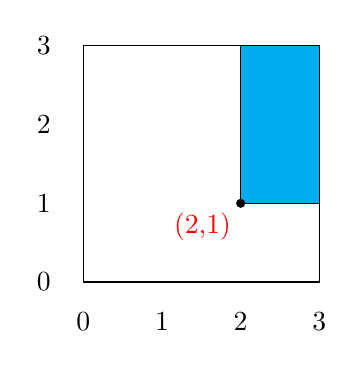
\begin{tikzpicture}
      \draw[step=1cm,black,thin] (0,0) rectangle (3,3);
      \foreach \xtick in {0,...,3} {\pgfmathsetmacro\result{\xtick * 1} \node at (\xtick,-0.5) {\pgfmathprintnumber{\result}}; }
      \foreach \ytick in {0,...,3} {\pgfmathsetmacro\result{\ytick * 1} \node at (-.5,\ytick) {\pgfmathprintnumber{\result}}; }
      \draw[fill=cyan] (2,1) rectangle (3,3);
      \draw [fill=black, thin] (2,1) circle [radius=0.05] node[below left,color=red]{(2,1)};
   \end{tikzpicture}
   \caption{Bottom-left corner example}
\end{figure}

\subsubsection*{Top-right corners} \label{sec:top-right-corners}
As \nameref{sec:bottom-left-corners} but representing the top-right corner of each rectangle (\texttt{tr\_corners}). It is used to reduce the number of positions in which a rectangle can fall in, because it must be inside the bounding box.

To reduce the search space, \texttt{tr\_corners} variables domain is defined as follows: $$\min({\min({px}), \min({py})}) \dots \max({h, w})$$

\begin{figure}[h]
   \centering
   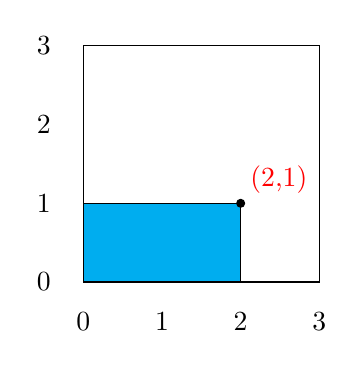
\begin{tikzpicture}
      \draw[step=1cm,black,thin] (0,0) rectangle (3,3);
      \foreach \xtick in {0,...,3} {\pgfmathsetmacro\result{\xtick * 1} \node at (\xtick,-0.5) {\pgfmathprintnumber{\result}}; }
      \foreach \ytick in {0,...,3} {\pgfmathsetmacro\result{\ytick * 1} \node at (-.5,\ytick) {\pgfmathprintnumber{\result}}; }
      \draw[fill=cyan] (0,0) rectangle (2,1);
      \draw [fill=black, thin] (2,1) circle [radius=0.05] node[above right,color=red]{(2,1)};
   \end{tikzpicture}
   \caption{Top-right corner example}
\end{figure}

\subsubsection*{Bottom-left corners values} \label{sec:bottom-left-corners-values}
This is a list of decision variables representing a linearization of bottom-left corners (\texttt{bl\_corners\_values}), which uses a one-to-one mapping from each two-dimensional coordinate in the bounding box to an integer value.

The mapping operates as follows:
$$ c: (x,y) \mapsto x+(y\cdot m),$$ where $m = \max{(h,w)}$.

To reduce the search space, \texttt{bl\_corners\_values} variables domain is defined as follows: $$0 \dots c(w, h)$$

\begin{figure}[h]
   \centering
   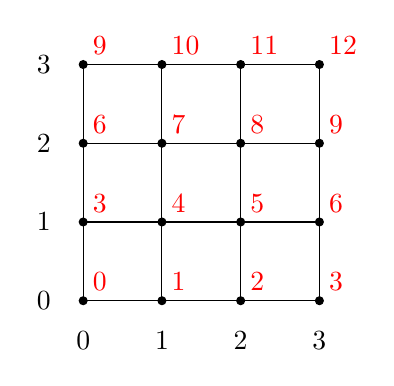
\begin{tikzpicture}
      \draw[step=1cm,black,thin] (0,0) grid (3,3);
      \foreach \xtick in {0,...,3} {\pgfmathsetmacro\result{\xtick * 1} \node at (\xtick,-0.5) {\pgfmathprintnumber{\result}}; }
      \foreach \ytick in {0,...,3} {\pgfmathsetmacro\result{\ytick * 1} \node at (-.5,\ytick) {\pgfmathprintnumber{\result}}; }
      \foreach \x in {0,...,3} {\foreach \y in {0,...,3} {\draw [fill=black, thin] (\x,\y) circle [radius=0.05] node[above right,color=red] {\pgfmathparse{\x+\y*3} \pgfmathprintnumber{\pgfmathresult}};}}
   \end{tikzpicture}
   \caption{Example of 2D-coordinates linearization in a 3 by 3 box}
\end{figure}

\subsection{Constraints}
The constraints described below, divided by scope, are presented at the top of each section with a simple schema depicting their evolution throughout different models.
The following is a legend explaining how constraints advancement is achieved:
\begin{itemize}
   \item \texttt{A[x]}: Constraint \texttt{A} has been introduced in model number \texttt{x}
   \item \texttt{A[x]} $\rightarrow$ \texttt{B[y]}: Constraint \texttt{A} was removed in favor of \texttt{B}, in model \texttt{y}
   \item \texttt{A[x]} $\rightarrow$ \xmark: Constraint \texttt{A} has not been carried over to models \texttt{x + 1, \dots}
\end{itemize}
Model numbers are related to their organization inside the attached Jupyter notebook.

\subsubsection{Non-overlapment}
\begin{itemize}
   \item \nameref{sec:presents-cannot-overlap} $\rightarrow$ \nameref{sec:diffnk}
   \item \nameref{sec:different-bl-corners}
\end{itemize}

\subsubsubsection{Presents cannot overlap [1]} \label{sec:presents-cannot-overlap}
The idea behind this simple constraint is, given a rectangle, to avoid the existance of areas of overlap with every other rectangle.
\begin{gather*}
   \max({bx_{i}, bx_{j}}) \geq \min({bx_{i} + px_{i}, bx_{j} + px_{j}}) \\
   \vee \\
   \max({by_{i}, by_{j}}) \geq \min({by_{i} + py_{i}, by_{j} + py_{j}}) \\
   \forall{i, j = 1 \dots n \mid j > i}
\end{gather*}

The described constraint has been observed to be efficient enough for relatively small instances of the problem, while already suffering to position rectangles in a $17 \times 17$ bounding box. Results are justified by the disjunctive nature of the constraint, which implies an higher burden in the propagation phase.

\subsubsubsection{Global \texttt{diffn\_k} [3]} \label{sec:diffnk}
The \texttt{diffn\_k} global constraint is defined by the official MiniZinc documentation \cite{minizinc} as follows: \\
\emph{Constrains k-dimensional boxes to be non-overlapping. For each box i and dimension j, box\_posn[i, j] is the base position of the box in dimension j, and box\_size[i, j] is the size in that dimension. Boxes whose size is 0 in any dimension still cannot overlap with any other box.}
\begin{verbatim}
   constraint diffn_k(bl_corners, presents);
\end{verbatim}
Being a global constraint, it gives a stronger propagation and a more efficient search w.r.t to \nameref{sec:presents-cannot-overlap}, allowing us to solve bigger instances, up to a $23 \times 23$ bounding box.

It's also notable, as described by \cite{sweep}, that \texttt{diffn\_k} is an onerous constraint. In \cite{sweep} it accounts for 30 to 80\% of the total running time, in an implementation of the \emph{PSP (Perfect Square Packing)} problem, which is very much related to \emph{PWP}.

\subsubsubsection{Global \texttt{all\_different} [2]} \label{sec:different-bl-corners}
The \texttt{all\_different} global constraint asserts that every variable has a different value assigned to it.

In our models it is used w.r.t \texttt{bl\_corners\_values} to ensure that every present has different \texttt{bl\_corners}. The choice of the constrained variables is related to their one-dimensional nature, which guarantees compatibility with MiniZinc's implementation of \texttt{all\_different}.
\begin{verbatim}
   constraint alldifferent(bl_corners_values);
\end{verbatim}

\subsubsection{Containment}
\begin{itemize}
   \item \nameref{sec:reduce-presents-domains}
   \item \nameref{sec:areas-summation}
\end{itemize}

\subsubsubsection{Reduce presents domains [1]} \label{sec:reduce-presents-domains}
The original description is the following one, where the lenght $l$ corresponds to the height \texttt{h\_paper} of the bounding box.:\\
\emph{In any solution, if we draw a vertical line and sum the vertical sides of the traversed pieces, the sum can be at most l. A similar property holds if we draw a horizontal line.}

As suggested by the assignment, we implemented this simple implied constraint which avoids pieces overflow in both directions.
\begin{gather*}
   bx_{i} \leq w + px_{i} \wedge by_{i} \leq h + py_{i}, \forall{i = 1 \dots n}
\end{gather*}

\subsubsubsection{Areas summation [4]} \label{sec:areas-summation}
This implied constraint is used to enforce presents to occupy the entire bounding box, without any kind of wasted space.
In particular, presents areas computed by using top-right and bottom-left corners are linked to the areas calculated using input pieces dimensions.

\begin{gather*}
   \sum_{i=1}^{n} (tx_{i} - bx_{i}) \cdot (ty_{i} - by_{i}) \leq w \cdot h
\end{gather*}
\begin{gather*}
   \sum_{i=1}^{n} (tx_{i} - bx_{i}) \cdot (ty_{i} - by_{i}) = \sum_{i=1}^{n} (px_{i} \cdot py_{i})
\end{gather*}

\subsubsection{Positioning}
\begin{itemize}
   \item \nameref{sec:present-at-origin}
   \item \nameref{sec:intervals-approach} $\rightarrow$ \xmark
   \item \nameref{sec:anchor-points-v1} $\rightarrow$ \nameref{sec:anchor-points-v2}$\rightarrow$ \xmark
\end{itemize}

\subsubsubsection{Global \texttt{count\_eq} [2]} \label{sec:present-at-origin}
This implied constraint exploits again the usage of bottom-left corners linearization, i.e. \texttt{bl\_corners\_values},
by stating that one and only one present should be placed with its bottom-left corner at the origin.

\begin{gather*}
   \lvert\{\,i \mid bx_{i} = 0 \wedge by_{i} = 0\,\}\rvert = 1
\end{gather*}

As mentioned in the section title, this idea has been implemented using the \texttt{count\_eq} global constraint.

\begin{verbatim}
   constraint count_eq(bl_corners_values, 0, 1);
\end{verbatim}

\subsubsubsection{Intervals approach [5]} \label{sec:intervals-approach}
It represents an idea taken from \cite{rect-packing}, where domains associated with the $x$-coordinate of bottom-left corners are reduced on the basis of a variable-sized interval:\\
\emph{[...] a rectangle is assigned an interval of x-coordinates. Interval sizes are hand-picked for each rectangle prior to search, and they induce a smaller rectangle representing the common intersecting area of placing the rectangle in any location in the interval. [...] we assign all x-coordinates prior to any y-coordinates, and use interval variables for the x-coordinates. We set a rectangle’s interval size to 0.35 times its width, which gave us the best performance. Finally, we do not use interval variables for the y-coordinates.}

\begin{figure}[h]
   \centering
   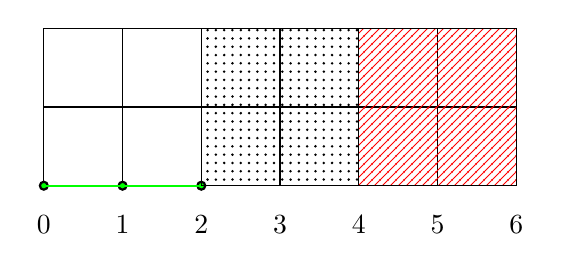
\begin{tikzpicture}
      \draw[step=1cm,black,thin] (0,0) grid (6,2);
      \foreach \xtick in {0,...,6} {\pgfmathsetmacro\result{\xtick * 1} \node at (\xtick,-0.5) {\pgfmathprintnumber{\result}}; }
      \draw[fill=green, thick] (0,0) circle [radius=0.05];
      \draw[fill=green, thick] (1,0) circle [radius=0.05];
      \draw[fill=green, thick] (2,0) circle [radius=0.05];
      \draw[color=green, thick] (0,0) -- (2,0);
      \draw[pattern=dots, pattern color=black] (2,0) rectangle (4,2);
      \draw[pattern=south west lines, pattern color=red] (4,0) rectangle (6,2);
   \end{tikzpicture}
   \caption{Intervals example: assigning $[0,2]$ to a $4\times2$ rectangle}
   \label{fig:intervals}
\end{figure}

As shown in figure \ref{fig:intervals}, a $4\times2$ rectangle assigned an $x$-interval of $[0,2]$ in a $6\times2$ box always consumes the units of area represented by the dotted rectangle,
while the rectangle containing red lines heading south west only has the possibility, and not the certainty, of being partially or totally consumed.
Moreover, the points on the green line represent the feasible assignments to the $x$-coordinate of the $4\times2$ rectangle's bottom-left corner.

In a more general situation, where the rectangle's height is less than the bounding box height, the $x$-interval reasoning remains the same, while the number of feasbile assignments to bottom-left corner's $y$-coordinate increases.

As a side note, the chosen interval in figure \ref{fig:intervals} has a size of $2$ because
$$ \lceil 4 \cdot 0.35 \rceil = \lceil 1.4 \rceil = 2,$$
where $4$ is the rectangle's width and $0.35$ is the selected parameter to compute interval sizes.

If there were no feasible set of interval assignments, then the constraint would save us from having to try individual $x$ values. However, if we do find a set of interval assignments, then we must search for a set of single $x$-coordinate values.

In the end, the implementation of this constraint didn't provide significant improvements. Hence, it is not present in the final CP model.

\subsubsubsection{Anchor points [5]} \label{sec:anchor-points-v1}
It represents a reduction on each present's domain, such that bottom-left corners reside on corners of other rectangles or on the wrapping paper borders.

The main implementation-wise problem was our inability of correctly expressing the constraint in an efficient way: the only thing we were able to describe is an upper bound on the number of the overall distinct corners that can be found inside the bounding box at the same time, while also satisfying every other constraint.
To do that, a new list of decision variables had to be created (\texttt{corners\_values}), containing the linearization (as in \ref{sec:bottom-left-corners-values}) of every corner for each present.
The constraint was then posted by limiting unique values, i.e. unique corners, over this new list of variables. Then, each bounding box corner was forced to coincide with exactly one value inside \texttt{corners\_values}.

\begin{verbatim}
   constraint nvalue(corners_values) <= 2 * n + 2
\end{verbatim}

The reported upper bound has been computed as follows:
\begin{theorem}
   Let $n$ be the number of rectangles to be placed inside a given squared bounding box.
   Let's assume that rectangles will completely fit inside the container, without free space.
   Then, we have that the number of distinct rectangles corners $k$ should be less than or equal to $2\cdot n + 2$.
\end{theorem}
\begin{proof}[Reasoning]
   Since we have $n$ rectangles, the total number of corners is exactly $4 \cdot n$. Moreover, we know that $4$ of these corners are reserved by the bounding box ones.
   For at least half of the other corners ($\frac{4 \cdot n - 4}{2}$), each one must be shared with at least two rectangles, because of our no-free-space assumption.
   By following this reasoning, we obtain these results:
   $$
      k \leq \frac{4 \cdot n - 4}{2} + 4 = 2\cdot n + 2 = u
   $$
\end{proof}

\begin{figure}[h]
   \centering
   \begin{subfigure}[b]{0.4\textwidth}
      \centering
      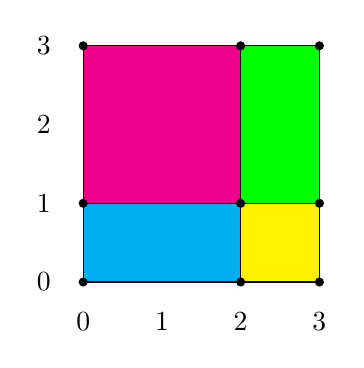
\begin{tikzpicture}
         \draw[step=1cm,black,thin] (0,0) rectangle (3,3);
         \foreach \xtick in {0,...,3} {\pgfmathsetmacro\result{\xtick * 1} \node at (\xtick,-0.5) {\pgfmathprintnumber{\result}}; }
         \foreach \ytick in {0,...,3} {\pgfmathsetmacro\result{\ytick * 1} \node at (-.5,\ytick) {\pgfmathprintnumber{\result}}; }
         \draw[fill=cyan] (0,0) rectangle (2,1);
         \draw[fill=magenta] (0,1) rectangle (2,3);
         \draw[fill=green] (2,1) rectangle (3,3);
         \draw[fill=yellow] (2,0) rectangle (3,1);
         \draw [fill=black, thin] (0,0) circle [radius=0.05];
         \draw [fill=black, thin] (2,0) circle [radius=0.05];
         \draw [fill=black, thin] (3,0) circle [radius=0.05];
         \draw [fill=black, thin] (0,1) circle [radius=0.05];
         \draw [fill=black, thin] (2,1) circle [radius=0.05];
         \draw [fill=black, thin] (3,1) circle [radius=0.05];
         \draw [fill=black, thin] (0,3) circle [radius=0.05];
         \draw [fill=black, thin] (2,3) circle [radius=0.05];
         \draw [fill=black, thin] (3,3) circle [radius=0.05];
      \end{tikzpicture}
      \caption{$k=9 \leq 10 =u$}
   \end{subfigure}
   \begin{subfigure}[b]{0.4\textwidth}
      \centering
      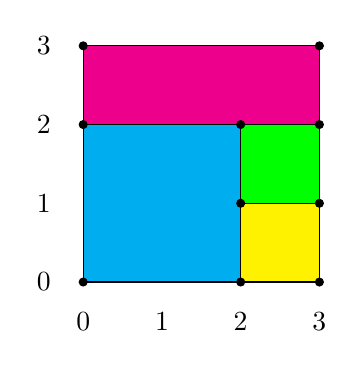
\begin{tikzpicture}
         \draw[step=1cm,black,thin] (0,0) rectangle (3,3);
         \foreach \xtick in {0,...,3} {\pgfmathsetmacro\result{\xtick * 1} \node at (\xtick,-0.5) {\pgfmathprintnumber{\result}}; }
         \foreach \ytick in {0,...,3} {\pgfmathsetmacro\result{\ytick * 1} \node at (-.5,\ytick) {\pgfmathprintnumber{\result}}; }
         \draw[fill=cyan] (0,0) rectangle (2,2);
         \draw[fill=magenta] (0,2) rectangle (3,3);
         \draw[fill=green] (2,1) rectangle (3,2);
         \draw[fill=yellow] (2,0) rectangle (3,1);
         \draw [fill=black, thin] (0,0) circle [radius=0.05];
         \draw [fill=black, thin] (2,0) circle [radius=0.05];
         \draw [fill=black, thin] (3,0) circle [radius=0.05];
         \draw [fill=black, thin] (2,1) circle [radius=0.05];
         \draw [fill=black, thin] (3,1) circle [radius=0.05];
         \draw [fill=black, thin] (0,2) circle [radius=0.05];
         \draw [fill=black, thin] (2,2) circle [radius=0.05];
         \draw [fill=black, thin] (3,2) circle [radius=0.05];
         \draw [fill=black, thin] (0,3) circle [radius=0.05];
         \draw [fill=black, thin] (3,3) circle [radius=0.05];
      \end{tikzpicture}
      \caption{$k=10 \leq 10 =u$}
   \end{subfigure}
   \caption{Distinct corners upper bound example}
\end{figure}

\subsubsubsection{Anchor points [6]} \label{sec:anchor-points-v2}
This constraint, taken from \cite{sweep} is an evolution of \nameref{sec:anchor-points-v1}, which introduces a more coincise and efficient anchor points approach.
This time the main idea is about causing the bottom-left corner of a single rectangle to fit a bottom-right or top-left corner of another already-placed rectangle, thus reducing the amount of available positions.

\begin{gather*}
   bx_{i} \in \{\,0\,\} \cup \{\, bx_{j} + px_{j} \mid j = 1 \dots i - 1, i + 1, \dots n \,\} \\
   \wedge \\
   by_{i} \in \{\,0\,\} \cup \{\, by_{j} + py_{j} \mid j = 1 \dots i - 1, i + 1, \dots n \,\} \\
   \forall{i = 1 \dots n}
\end{gather*}

The described formula was implemented using the global constraint \texttt{member}, so as to achieve better propagation.

The constraint was later removed from the CP model, since it didn't seem to make any major difference, at least w.r.t. running times over the test instances, even though it was implemented using the mentioned global constraint.

\begin{figure}[h]
   \centering
   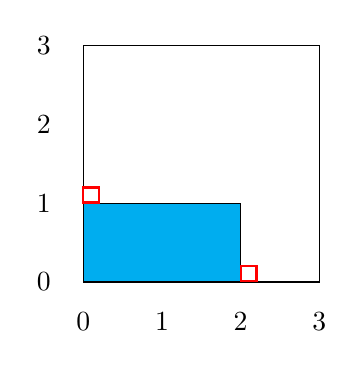
\begin{tikzpicture}
      \draw[step=1cm,black,thin] (0,0) rectangle (3,3);
      \foreach \xtick in {0,...,3} {\pgfmathsetmacro\result{\xtick * 1} \node at (\xtick,-0.5) {\pgfmathprintnumber{\result}}; }
      \foreach \ytick in {0,...,3} {\pgfmathsetmacro\result{\ytick * 1} \node at (-.5,\ytick) {\pgfmathprintnumber{\result}}; }
      \draw[fill=cyan] (0,0) rectangle (2,1);
      \draw[color=red, thick] (2,0.01) rectangle (2.2,0.2);
      \draw[color=red, thick] (0,1.01) rectangle (0.2,1.2);
   \end{tikzpicture}
   \caption{Anchor points example}
   \label{fig:anchor-points}
\end{figure}

Figure \ref{fig:anchor-points} shows the available placements of a rectangle, different than the one filled in cyan,
which could be positioned in such a way that its bottom-left corner would overlap with one of the two small red rectangles.

\subsubsection{Stacking}
\begin{itemize}
   \item \nameref{sec:cumulative}
   \item \nameref{sec:stack-two} $\rightarrow$ \nameref{sec:column-stacking}
\end{itemize}

\subsubsubsection{Global \texttt{cumulative} [3]} \label{sec:cumulative}
The \texttt{cumulative} global constraint is defined by the official MiniZinc documentation \cite{minizinc} as follows: \\
\emph{Requires that a set of tasks given by start times s, durations d, and resource requirements r, never require more than a global resource bound b at any one time.}

\begin{verbatim}
   constraint cumulative(
      bl_corners_xs, presents_xs, presents_ys, h_paper
   );
   constraint cumulative(
      bl_corners_ys, presents_ys, presents_xs, w_paper
   );
\end{verbatim}

In the context of rectangle packing, the cumulative global constraint can be used by selecting $x$-coordinates of bottom-left corners as start times, by assigning durations to presents widths, resource requirements to presents heights and the global resource bound to the paper roll height.
The same reasoning can be applied for the other dimension, in order to obtain overflow avoidance and stacking maximization over both axis.

\begin{figure}[h]
   \centering
   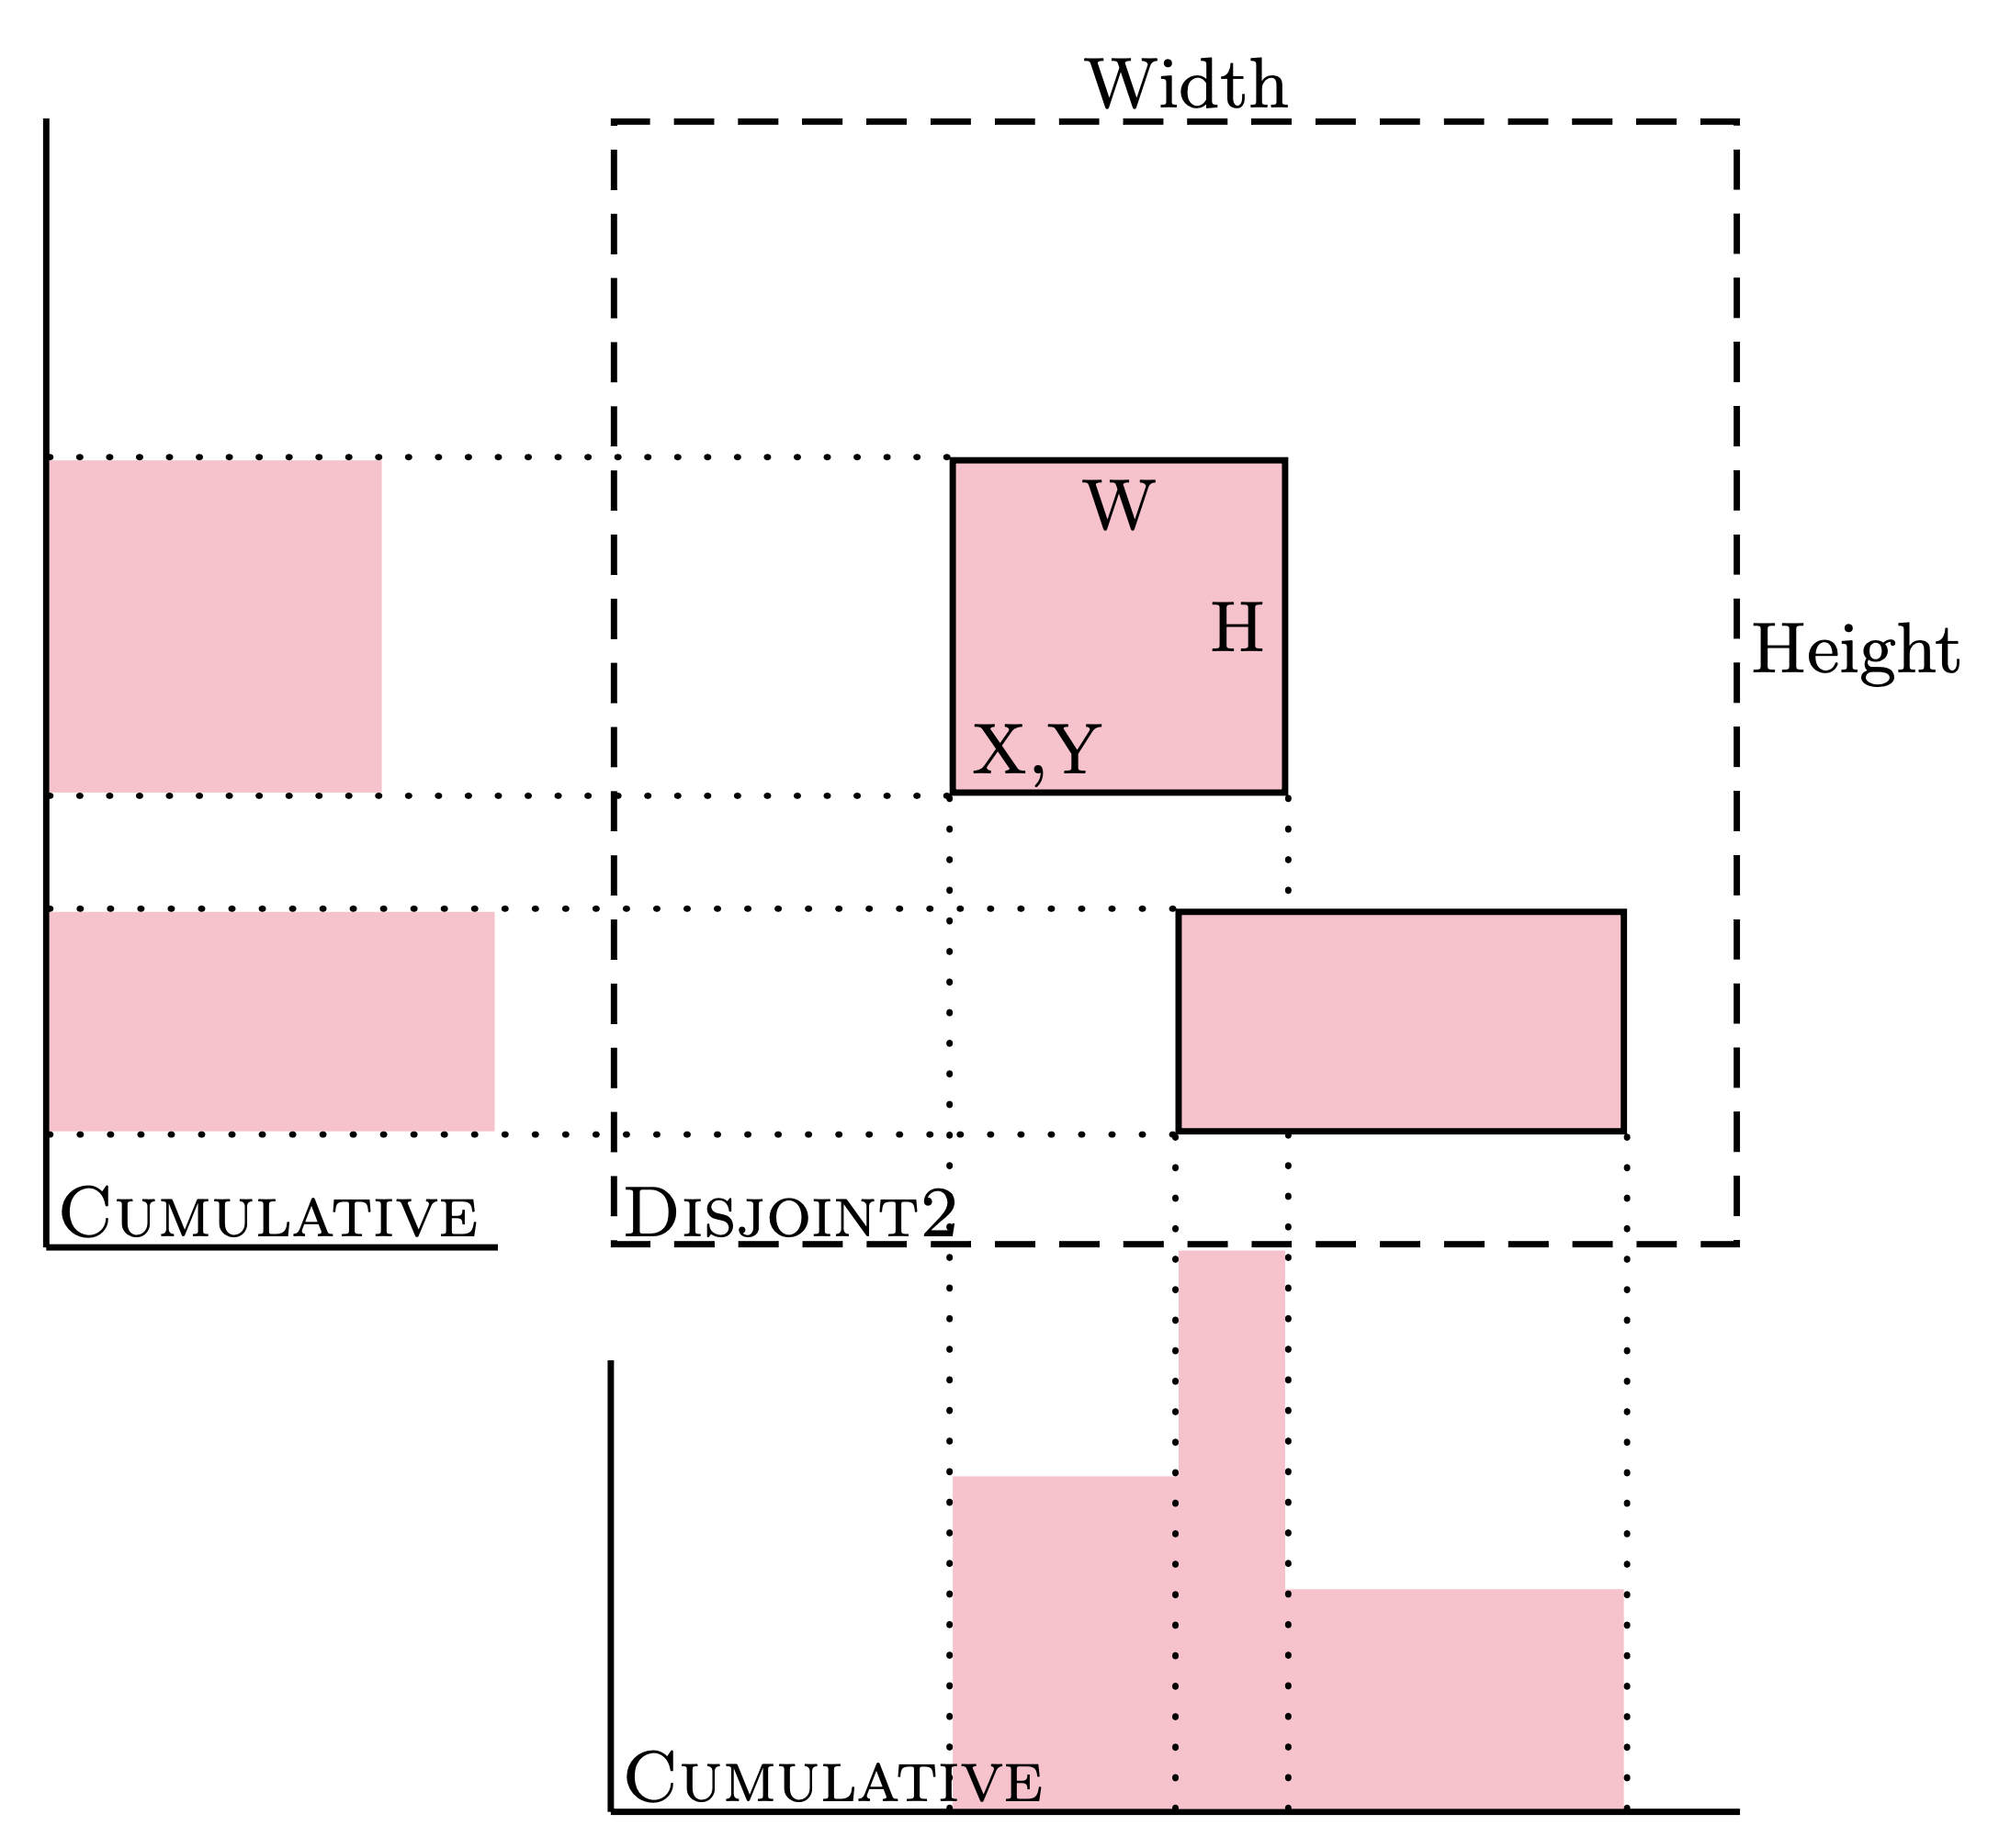
\includegraphics[scale=0.2]{cumulative.png}
   \caption{Cumulative global constraint (image taken from \cite{cumulative})}
   \label{fig:cumulative}
\end{figure}

Figure \ref{fig:cumulative} shows an example of the \texttt{cumulative} global constraint, along with the usage of \texttt{disjoint2}, which is the twin constraint of the already mentioned \texttt{diffn\_k}.

The combination of \texttt{cumulative} and \texttt{diffn\_k} is actually the core of the CP model, since together they enable a very strong propagation, which can be directly observed by looking at solving times.

\subsubsubsection{Column stacking by two [4]} \label{sec:stack-two}
The main idea behind this simple constraint is to stack presents in a single row or column such that their widths or heights would sum to the total width or height, respectively, of the entire paper roll.

\begin{figure}[h]
   \centering
   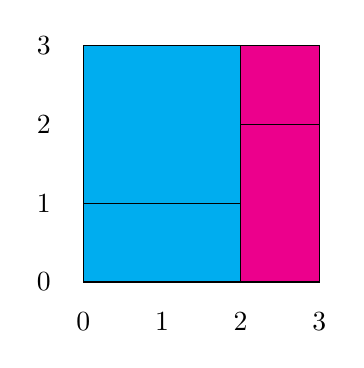
\begin{tikzpicture}
      \draw[step=1cm,black,thin] (0,0) rectangle (3,3);
      \foreach \xtick in {0,...,3} {\pgfmathsetmacro\result{\xtick * 1} \node at (\xtick,-0.5) {\pgfmathprintnumber{\result}}; }
      \foreach \ytick in {0,...,3} {\pgfmathsetmacro\result{\ytick * 1} \node at (-.5,\ytick) {\pgfmathprintnumber{\result}}; }
      \draw[fill=cyan] (0,0) rectangle (2,1);
      \draw[fill=cyan] (0,1) rectangle (2,3);
      \draw[fill=magenta] (2,0) rectangle (3,2);
      \draw[fill=magenta] (2,2) rectangle (3,3);
   \end{tikzpicture}
   \caption{Column stacking by two example}
   \label{fig:col-stacking-two}
\end{figure}

In figure \ref{fig:col-stacking-two}, we can observe two different groups, the cyan and the magenta one. In this example, we are stacking by columns, since each color group contains rectangles with the same width and such that their heights sum to the total bounding box height.

When the constraint is applied, both rectangles must have the same $x$-coordinate for bottom-left corners, while the $y$-coordinate is assigned to zero for the "first" rectangle and to the height of the first present for the "second" rectangle.

\subsubsubsection{General column stacking [5]} \label{sec:column-stacking}
This constraint is a generalization of the simpler \nameref{sec:stack-two}, which introduces packing multiple rectangles, i.e. groups of size greater than two, into multiple columns.

\begin{figure}[h]
   \centering
   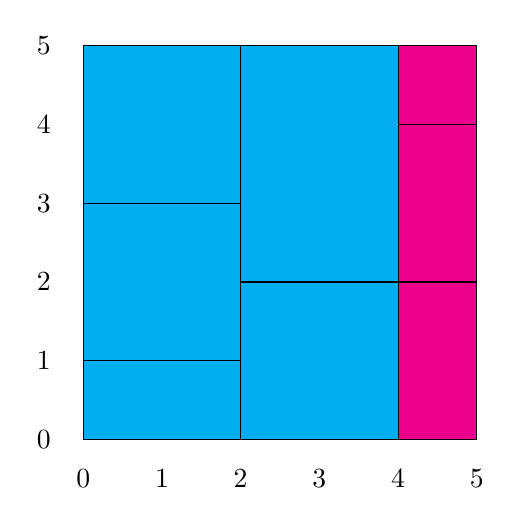
\begin{tikzpicture}
      \draw[step=1cm,black,thin] (0,0) rectangle (5,5);
      \foreach \xtick in {0,...,5} {\pgfmathsetmacro\result{\xtick * 1} \node at (\xtick,-0.5) {\pgfmathprintnumber{\result}}; }
      \foreach \ytick in {0,...,5} {\pgfmathsetmacro\result{\ytick * 1} \node at (-.5,\ytick) {\pgfmathprintnumber{\result}}; }
      \draw[fill=cyan] (0,0) rectangle (2,1);
      \draw[fill=cyan] (0,1) rectangle (2,3);
      \draw[fill=cyan] (0,3) rectangle (2,5);
      \draw[fill=cyan] (2,0) rectangle (4,2);
      \draw[fill=cyan] (2,2) rectangle (4,5);
      \draw[fill=magenta] (4,0) rectangle (5,2);
      \draw[fill=magenta] (4,2) rectangle (5,4);
      \draw[fill=magenta] (4,4) rectangle (5,5);
   \end{tikzpicture}
   \caption{General column stacking example}
   \label{fig:col-stacking}
\end{figure}

This predicate is subdivided into different steps:
\begin{itemize}
   \item Groups identification: finds and groups together presents with the same width
   \item Feasibility check: ensures that every group can occupy at least one entire column
   \item Columns computation: calculates the number of columns (and the corresponding widths) occupied by each group (e.g. a group of width $2$ with heights $[1,2,3]$ in a $12\times3$ box will occupy exactly two columns of width $2$)
   \item Columns/coordinates assignment: using the \texttt{bin\_packing} global constraint to identify the column for each rectangle in the same group, it incrementally fixes $x$ and $y$ bottom-left corners coordinates
\end{itemize}

Groups are ordered by decreasing widths, while rectangles in the same group are sorted by decreasing heights.

In figure \ref{fig:col-stacking} we can see how the entire group of cyan-filled rectangles, which has a common width of $2$, gets splitted into subsequent columns, while the magenta-colored group can only occupy one column, the last one in this example.

\subsubsection{Symmetry breaking}
\begin{itemize}
   \item \nameref{sec:biggest-lower-left} $\rightarrow$ \nameref{sec:areas-ordering}
   \item \nameref{sec:width-ordering} $\rightarrow$ \xmark
\end{itemize}

\subsubsubsection{Biggest rectangle in lower left quadrant [4]} \label{sec:biggest-lower-left}
Inspired by the standard n-queens problem, we tried to analyze PWP and its solutions, obtained by reflecting axes.

To cut the search space and avoid exploring paths leading to symmetric non-solutions, we decided to force the biggest rectangle, i.e. the one with greatest area, to have its bottom-left corner inside the lower-left quadrant of the bounding box.

\begin{figure}[h]
   \centering
   \begin{subfigure}[b]{0.4\textwidth}
      \centering
      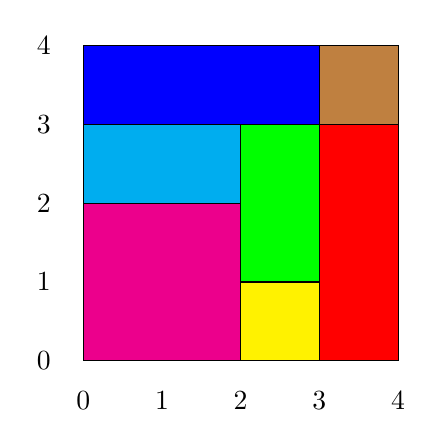
\begin{tikzpicture}
         \draw[step=1cm,black,thin] (0,0) rectangle (4,4);
         \foreach \xtick in {0,...,4} {\pgfmathsetmacro\result{\xtick * 1} \node at (\xtick,-0.5) {\pgfmathprintnumber{\result}}; }
         \foreach \ytick in {0,...,4} {\pgfmathsetmacro\result{\ytick * 1} \node at (-.5,\ytick) {\pgfmathprintnumber{\result}}; }
         \draw[fill=cyan] (0,2) rectangle (2,3);
         \draw[fill=magenta] (0,0) rectangle (2,2);
         \draw[fill=green] (2,1) rectangle (3,3);
         \draw[fill=yellow] (2,0) rectangle (3,1);
         \draw[fill=red] (3,0) rectangle (4,3);
         \draw[fill=blue] (0,3) rectangle (3,4);
         \draw[fill=brown] (3,3) rectangle (4,4);
      \end{tikzpicture}
      \caption{Original solution}
      \label{fig:symmetry-a}
   \end{subfigure}
   \begin{subfigure}[b]{0.4\textwidth}
      \centering
      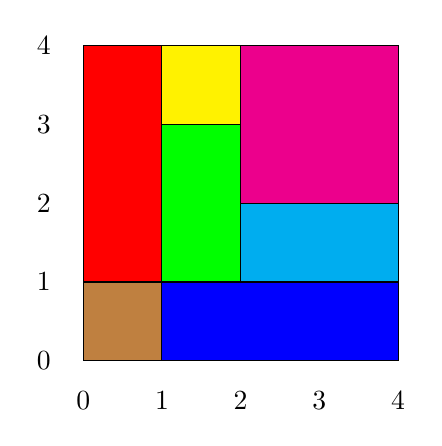
\begin{tikzpicture}
         \draw[step=1cm,black,thin] (0,0) rectangle (4,4);
         \foreach \xtick in {0,...,4} {\pgfmathsetmacro\result{\xtick * 1} \node at (\xtick,-0.5) {\pgfmathprintnumber{\result}}; }
         \foreach \ytick in {0,...,4} {\pgfmathsetmacro\result{\ytick * 1} \node at (-.5,\ytick) {\pgfmathprintnumber{\result}}; }
         \draw[fill=cyan] (2,1) rectangle (4,2);
         \draw[fill=magenta] (2,2) rectangle (4,4);
         \draw[fill=green] (1,1) rectangle (2,3);
         \draw[fill=yellow] (1,3) rectangle (2,4);
         \draw[fill=red] (0,1) rectangle (1,4);
         \draw[fill=blue] (1,0) rectangle (4,1);
         \draw[fill=brown] (0,0) rectangle (1,1);
      \end{tikzpicture}
      \caption{Reflected solution}
      \label{fig:symmetry-b}
   \end{subfigure}
   \caption{Symmetric solutions example}
   \label{fig:symmetry}
\end{figure}

Figure \ref{fig:symmetry} depicts an example of specular solutions, s.t. subfigure \ref{fig:symmetry-a} satisfies the constraint, while \ref{fig:symmetry-b} does not.

In the end, we realized that this approach was too limiting, thus leading to an increase in the number of failures. Because of this, we decided to remove it in favor of \nameref{sec:areas-ordering}.

\subsubsubsection{Ordering by areas [6]} \label{sec:areas-ordering}
This constraint is based on \cite{sweep} and it is used to create a lexicographical ordering between the bottom-left corners coordinates of the biggest rectangle $r_{1}$, i.e. the one with the greatest area, and the coordinates of the second biggest present $r_{2}$.
In this way, $r_{1}$ must be placed below and/or to the left of $r_{2}$.

\begin{verbatim}
   lex_less(
      [bl_corners_ys[r1], bl_corners_xs[r1]],
      [bl_corners_ys[r2], bl_corners_xs[r2]]
   );
\end{verbatim}

Implementation-wise, we decided to use the global constraint \texttt{lex\_less}, as shown above.

\subsubsubsection{In-column ordering by width [4]} \label{sec:width-ordering}
This was our first try to enable some kind of ordering between presents with the same bottom-left corners $x$-coordinates.
In particular, those presents which happen to have the same $x$-coordinate will be constrained to be ordered by their heights s.t. smaller pieces would lie below the taller ones.

Results were not good at all, since this approach transformed a subset of solvable instances into unfeasible ones, because it was highly dependent on input presents order. Hence, the constraint is not present in the final model.

\subsection{Models}
In this section are presented our final models and their search strategy. The optional model has the ability to handle presents rotation and rectangles with the same shapes.
\subsubsection*{Search strategy}
We decided to prioritize positioning "bigger" presents first, since their placement greatly reduce the domain of the other ones. After trying every meaningful ordering, i.e. by height, width or area, the one that gave us the best outcomes was sorting presents by decreasing values of area.

\begin{verbatim}
   array[1..n] of int: areas =
      [presents_xs[i] * presents_ys[i] | i in 1..n];
   array[1..n] of 1..n: order =
      sort_by(1..n, [-areas[i] | i in 1..n]);
\end{verbatim}

The actual search strategy starts by checking if \nameref{sec:column-stacking} is feasible. In case of a positive answer we do not need to apply complex approaches, since everything is already handled by column stacking positioning. On the other hand, when column stacking is not feasible, we rely on the previously defined ordering by assigning firstly $y$-coordinates and then $x$-coordinates. These assignments are done by selecting values starting from the minimum one in each domain.

In this kind of search strategy applying restarts was not an option, since we didn't have any random component. Anyway we tried to use \texttt{luby} and \texttt{constant} restarts in a simpler search strategy, but it resulted into worse running times.

\begin{verbatim}
   solve::
    if not(col_stacking_feasible) then
        seq_search([
            int_search(
               [bl_corners_ys[i] | i in order],
               input_order,
               indomain_min,
               complete
            ),
            int_search(
               [bl_corners_xs[i] | i in order],
               input_order,
               indomain_min,
               complete
            )
        ])
    else
      int_search(
         bl_corners_values,
         dom_w_deg,
         indomain_min,
         complete
      )
    endif
   satisfy;
\end{verbatim}

\subsubsection*{Final model}
To present a global undestanding of our final model, below we report a list linking to each and every included constraint.
\begin{itemize}
   \item \nameref{sec:diffnk}
   \item \nameref{sec:cumulative}
   \item \nameref{sec:reduce-presents-domains}
   \item \nameref{sec:different-bl-corners}
   \item \nameref{sec:present-at-origin}
   \item \nameref{sec:areas-summation}
   \item \nameref{sec:areas-ordering}
   \item \nameref{sec:column-stacking}
\end{itemize}
Using this model we were able to solve every test instance, with the exception of the $23\times23$ one, in under one second. This was mostly possible thanks to the \nameref{sec:column-stacking} constraint, which enabled us to reduce running times, in particular w.r.t. bigger instances.

\begin{figure}[h]
   \centering
   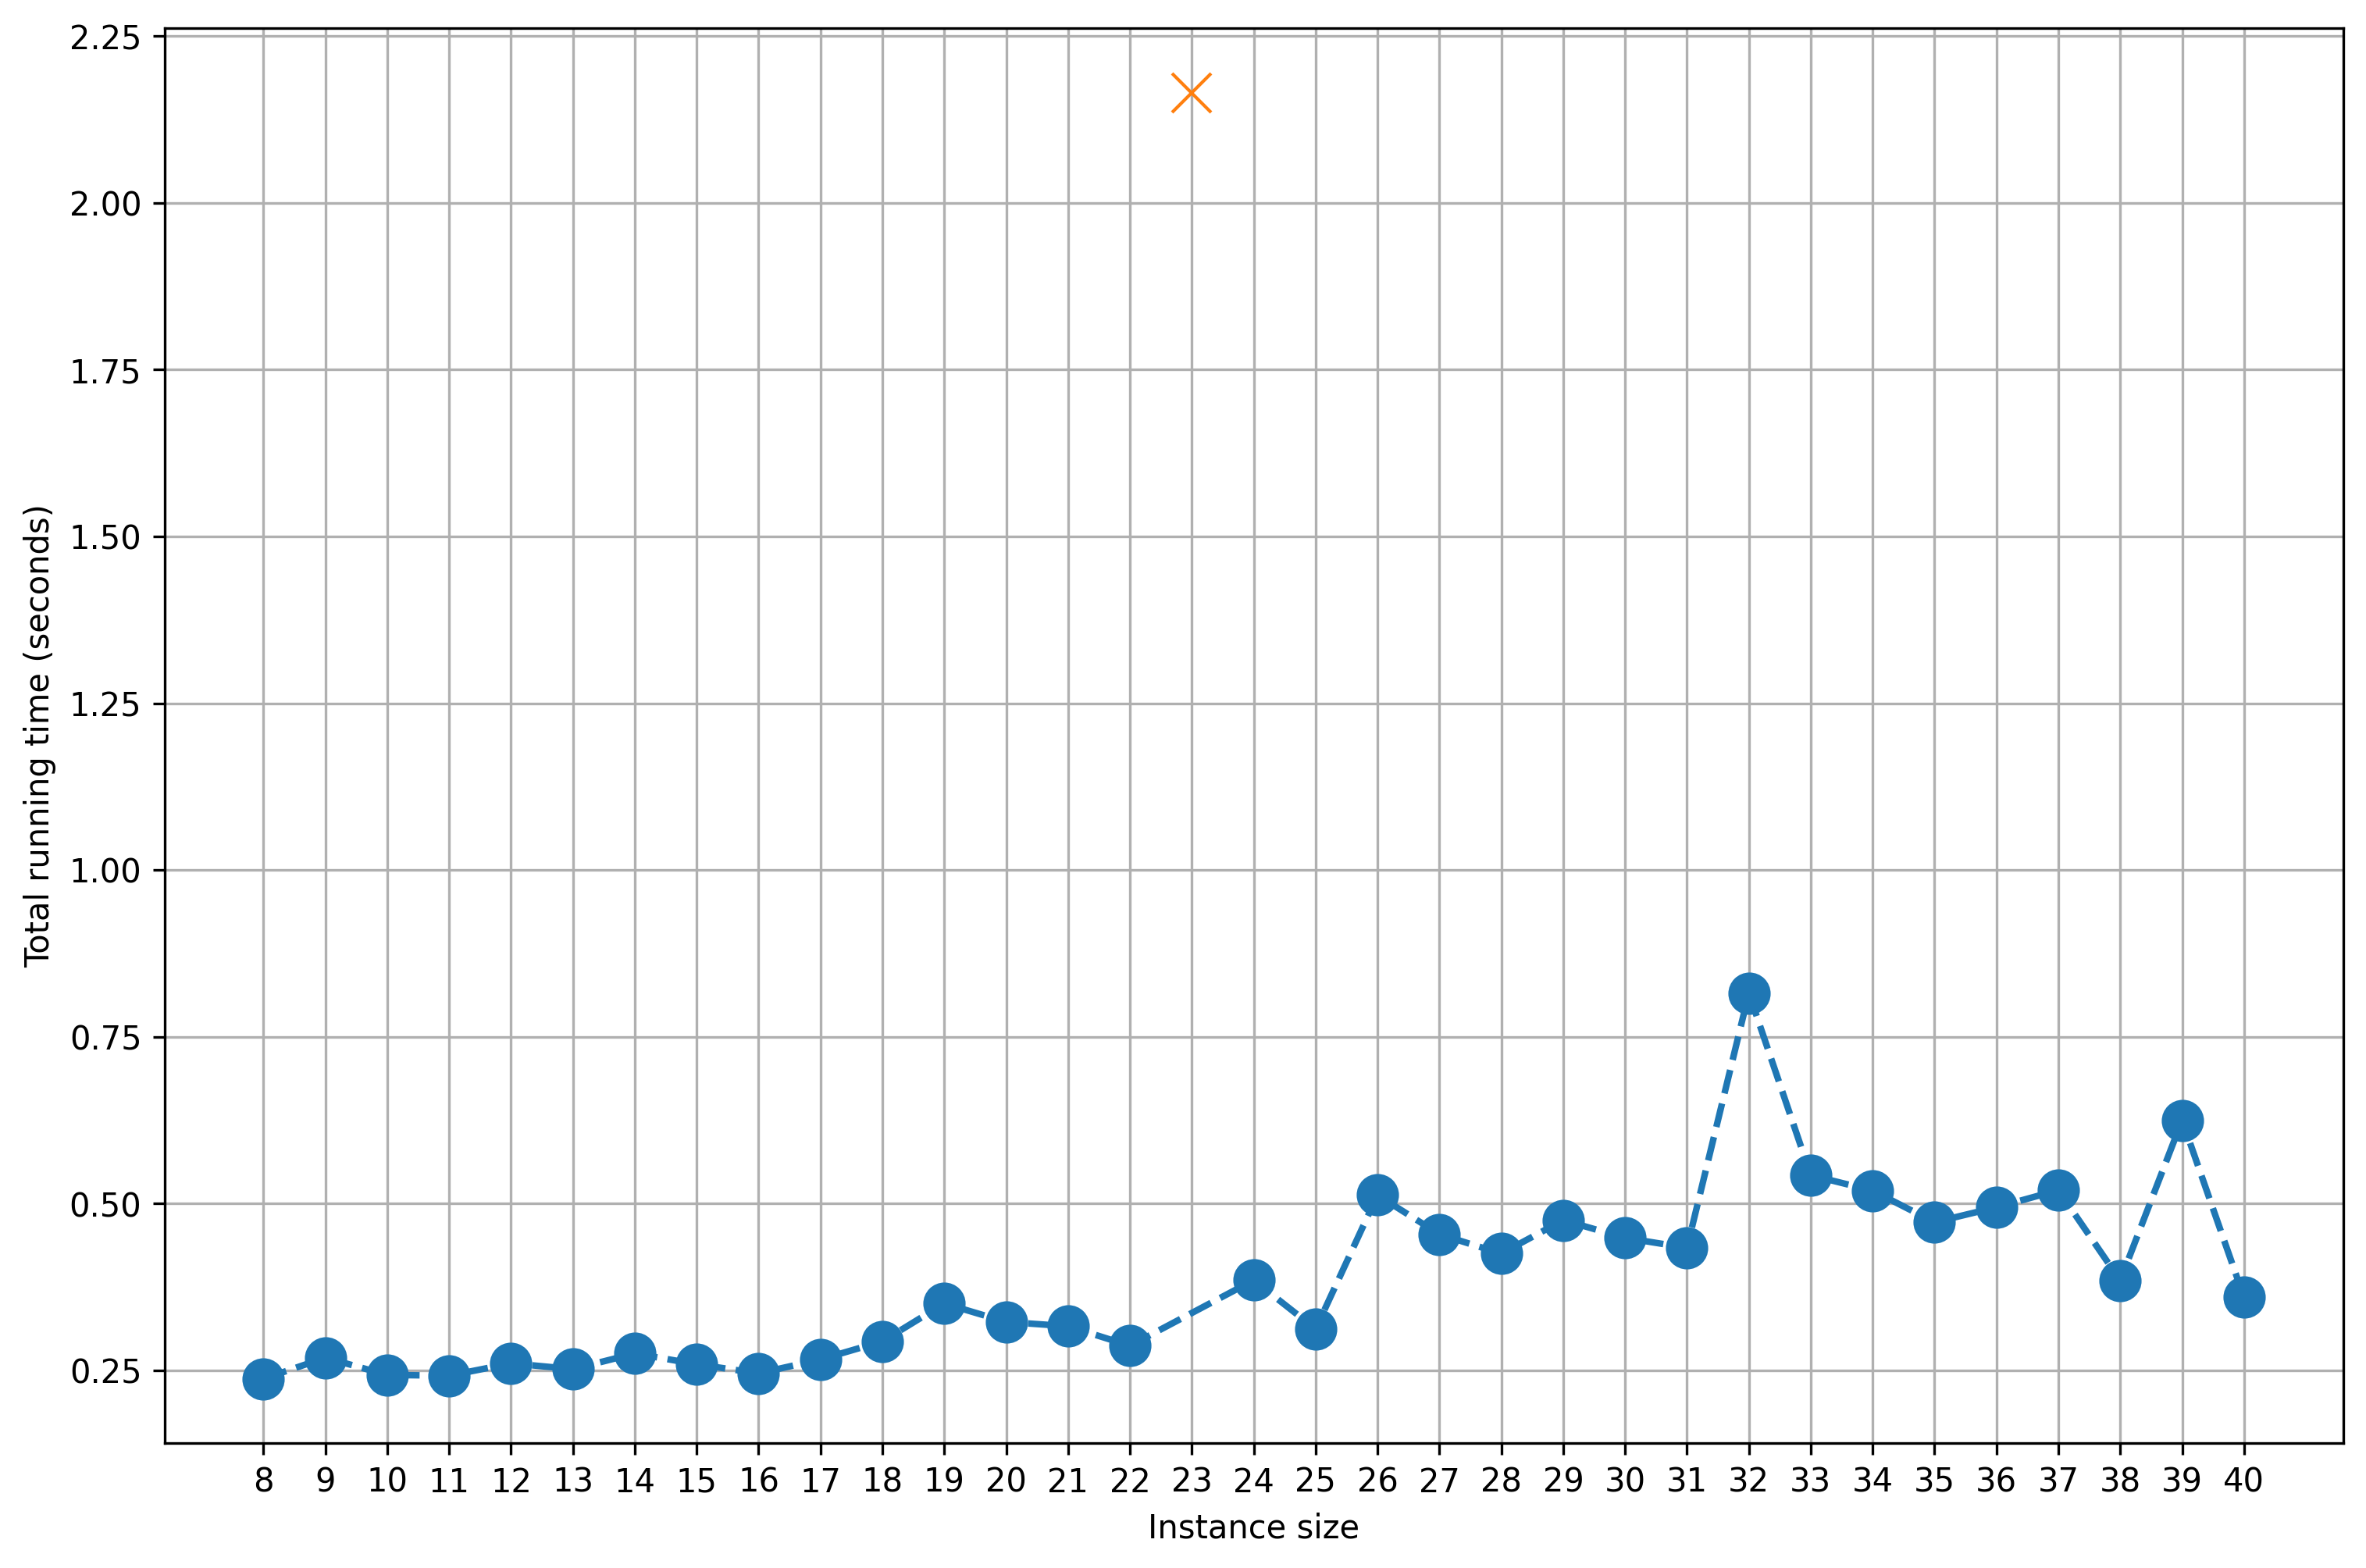
\includegraphics[scale=0.45]{cp-times.png}
   \caption{Final CP model running times}
\end{figure}

\subsubsection*{Optional model}
This model is dedicated to the implementation of the optional parts of the project, namely rotation and same dimensions handling.

About rotation, we removed the column stacking approach, since presents dimensions are now considered as variables, and we introduced the global constraint \texttt{geost\_bb} which can be used to find appropriate positions and rotations of the given rectangles without overlaps, by constraining them to be contained in a given bounding box. This approach obviously turned out to be much slower w.r.t. our final model.

The \texttt{geost\_bb} global constraint is defined by the official MiniZinc documentation \cite{minizinc} as follows: \\
\emph{A global non-overlap constraint for k dimensional objects. It enforces that no two objects overlap, and that all objects fit within a global k dimensional bounding box.}

\begin{verbatim}
   constraint geost_bb(
      k, rect_size, rect_offset, shape, bl_corners, kind, l, u
   );
\end{verbatim}

About \texttt{geost\_bb} parameters, as described in \cite{geost}:
\begin{itemize}
   \item \texttt{k}: The number of dimensions, i.e. 2
   \item \texttt{rect\_size}: The size of each rectangle in \texttt{k} dimensions, i.e. a list of $2\cdot n$ elements given by the dimensions of each present and its $90^{\circ}$ rotation
   \item \texttt{rect\_offset}: The offset of each rectangle from the base position in \texttt{k}  dimensions, i.e. a list of $2\cdot n$ elements fixed to $[0,0]$, representing the offset of each rectangle from the top-right corner of its minimum enclosing bounding-box
   \item \texttt{shape}: The set of rectangles defining the $i$-th shape, i.e.a list of $2\cdot n$ indexes going from $1$ to $2\cdot n$, representing that each figure is directly associated with exactly one rectangle
   \item \texttt{bl\_corners}: The base position of each object
   \item \texttt{kind}: A list of $n$ elements, representing the shape used by each object, i.e. either the original rectangle or its $90^{\circ}$ rotation
   \item \texttt{l}: An array of lower bounds, i.e. the bottom-left corner of our paper roll
   \item \texttt{u}: An array of upper bounds, i.e. the top-right corner of our paper roll.
\end{itemize}

In order to achieve better results, it could be possible to find the minimum number of rotations needed to make column stacking feasible and proceed like before.

About rectangles with same dimensions, we simply included a symmetry breaking constraint accounting for pairwise positioning of equally-sized presents, because these presents can be swapped without any kind of difference in the results.

\begin{verbatim}
   constraint forall(i in 1..n)(
      let {
          array[int] of int: same_dim_ind = [
               j | j in 1..n where
               presents_xs[j] = presents_xs[i] /\
               presents_ys[j] = presents_ys[i]
            ]
      } in
          if
            length(same_dim_ind) > 1 /\
            min(same_dim_ind) = i
          then
            forall(j in index_set(same_dim_ind) where j > 1) (
               lex_less(
                  [
                     bl_corners_ys[same_dim_ind[j - 1]],
                     bl_corners_xs[same_dim_ind[j - 1]]
                  ],
                  [
                     bl_corners_ys[same_dim_ind[j]],
                     bl_corners_xs[same_dim_ind[j]]
                  ]
               )
            )
          else true
          endif
  );
\end{verbatim}

The above code groups rectangles with the same dimensions and constrains the one with the minimum index to be placed below and/or to the left of the second one; the same happens between the second and the third presents in the same group; and so on and so forth. This approach creates a chain of constraints s.t. every symmetric solution and non-solution is eliminated from the search path.

\section{Satisfiability Modulo Theory}

\printbibliography

\end{document}
